\documentclass[10.5pt]{article}

% ---- geometry & general ----
\usepackage[a4paper,margin=0.82in]{geometry}
\usepackage[T1]{fontenc}
\usepackage{mathpazo}
\usepackage{microtype}
\usepackage{titlesec}
\usepackage{fancyhdr}
\usepackage{booktabs}
\usepackage{array}
\usepackage{graphicx}
\usepackage{caption}
\usepackage{enumitem}
\usepackage{amsmath}
\usepackage{amssymb}
\usepackage{textcomp}
\usepackage{xcolor}
\usepackage{adjustbox}
\usepackage{tcolorbox}
\tcbuselibrary{skins,breakable}
\usepackage{pgfplots}
\pgfplotsset{compat=1.16}
\usepackage{tikz}
\usetikzlibrary{arrows.meta,positioning,patterns}
\usepackage[hidelinks]{hyperref}

% ---- pure black/white/gray palette ----
\definecolor{inkblack}{RGB}{0,0,0}
\definecolor{lightgray}{RGB}{228,228,228}
\definecolor{g1}{gray}{0.80}
\definecolor{g2}{gray}{0.66}
\definecolor{g3}{gray}{0.52}
\definecolor{g4}{gray}{0.40}
\definecolor{g5}{gray}{0.27}
\definecolor{g6}{gray}{0.13}
\hypersetup{colorlinks=true, linkcolor=inkblack, citecolor=inkblack, urlcolor=inkblack,
  pdftitle={Cache-Aware Optimisation of the ESKAPE Nanopore Pipeline},
  pdfauthor={Chirag Kathpalia, Chirag Suthar}}
\color{inkblack}

% ---- grayscale chart style ----
\pgfplotsset{
  grayaxis/.style={
    font=\footnotesize, tick align=outside, grid=major,
    major grid style={line width=.25pt, draw=black!14},
    axis line style={draw=black!70, line width=.5pt},
    tick style={draw=black!70},
    label style={font=\footnotesize}, tick label style={font=\scriptsize},
    legend style={font=\scriptsize, draw=black!40, fill=white, rounded corners=1pt},
  }
}

% ---- headings ----
\titleformat{\section}{\normalfont\large\bfseries}{\thesection}{0.55em}{}
\titleformat{\subsection}{\normalfont\normalsize\bfseries}{\thesubsection}{0.55em}{}
\titlespacing*{\section}{0pt}{1.1em}{0.55em}
\titlespacing*{\subsection}{0pt}{0.85em}{0.35em}

% ---- header/footer ----
\pagestyle{fancy}
\fancyhf{}
\renewcommand{\headrulewidth}{0.4pt}
\renewcommand{\footrulewidth}{0.2pt}
\fancyhead[L]{\footnotesize\textsc{ESKAPE Nanopore Pipeline}}
\fancyhead[R]{\footnotesize\textsc{Cache-Aware Optimisation of Kraken2}}

\fancyfoot[C]{\footnotesize\thepage}
\fancyfoot[R]{\footnotesize Summer 2026}

\captionsetup{labelfont=bf,font=footnotesize,labelsep=period,justification=raggedright,singlelinecheck=false}

\newcommand{\code}[1]{\texttt{\footnotesize #1}}
\newenvironment{honestbox}[1]{%
  \begin{tcolorbox}[breakable,boxrule=0.6pt,colframe=inkblack,colback=white,
    left=7pt,right=7pt,top=5pt,bottom=5pt,arc=0pt,before skip=8pt,after skip=8pt,
    title={\footnotesize\bfseries #1},fonttitle=\footnotesize,coltitle=inkblack,
    colbacktitle=lightgray,boxsep=2pt]
}{\end{tcolorbox}}

\setlength{\parskip}{0.42em}
\setlength{\parindent}{0pt}
\setlength{\emergencystretch}{2.5em}
\linespread{1.02}

\begin{document}

% ================= COMPACT HEADER =================
\begin{center}
{\LARGE\bfseries Cache-Aware Optimisation of Kraken2\\[0.14cm] Classification for the ESKAPE Nanopore Pipeline}\\[0.35cm]
{\normalsize Minor Project Report - the \textit{kraken2opti} track, with cross-hardware profiling}\\[0.4cm]
{\small Chirag Kathpalia \quad $\cdot$ \quad Chirag Suthar}\\[0.1cm]
{\small under the guidance of \textbf{Prof.\ Kolin Paul} \quad $\vert$ \quad Department of Computer Science and Engineering, IIT Delhi}\\[0.1cm]
{\small Summer 2026}
\end{center}

\vspace{0.25cm}
\noindent\rule{\textwidth}{0.4pt}
\vspace{0.1cm}

{\small\textbf{Abstract.} Oxford Nanopore metagenomics for ESKAPE pathogen identification runs a two-stage pipeline: \textbf{Dorado}, a GPU neural basecaller, and \textbf{Kraken2}, a CPU k-mer classifier. Profiling across three machines places the two stages on opposite sides of the compute/memory roofline: Dorado is compute-bound and already runs its GPU at physical capacity (97.6--99.5\% SM utilisation), while Kraken2's random-probe lookup \code{CompactHashTable::Get()} accounts for 96.24\% of last-level-cache read misses despite only 0.65\% of instructions, it is memory-latency-bound, and the lever that matters is the database's memory footprint. The implemented contribution narrows Kraken2's compact-hash cell width from the stock 32 bits to 24 and 16 bits, cutting an ESKAPE-panel database by 25\% and 50\%. An exponential false-positive law, $\mathrm{FP}\!\approx\!p\,2^{-b}$, predicts a sharp accuracy cliff at $\approx$13 check bits and proves 24-bit is a lossless drop-in, while 16-bit reaches equivalent accuracy once a small confidence threshold suppresses collisions. A 1{,}728-run cross-hardware sweep confirms the cliff on independent data.}

\vspace{0.1cm}
\noindent\rule{\textwidth}{0.4pt}

% ================= SECTION 1 : INTRODUCTION =================
\section{Introduction}

Oxford Nanopore metagenomics for ESKAPE pathogen identification runs a two-stage pipeline. a neural basecaller (Dorado~\cite{dorado})  converts the raw ionic-current squiggle from a nanopore flow cell into DNA reads on the GPU, and a classifier (Kraken2~\cite{kraken2}) assigns every read to a taxon by reducing it to a set of \textit{minimizers}~\cite{minimizers} and matching each against a reference \textit{compact hash table} (CHT). the target organisms are six antibiotic-resistant \textbf{ESKAPE pathogens}~\cite{eskape}  \textit{E.\,faecium, S.\,aureus, K.\,pneumoniae, A.\,baumannii, P.\,aeruginosa, E.\,cloacae} - a panel known in advance, where fast and low-memory turnaround matters for point-of-care and edge deployment.

the reason to optimise the classification stage, not basecalling, is a memory-hierarchy mismatch. Kraken2's lookup is an exact-match probe~\cite{kraken1} into a hash table orders of magnitude larger than any CPU cache, so essentially every probe misses cache and pays full DRAM latency; the stage is bound by \textit{memory footprint}, not arithmetic. a smaller database therefore classifies faster and keeps more of its working set cache-resident. the specific opening this report exploits is that a six-organism panel needs only a handful of taxon bits, so most of each 32-bit CHT cell is spent collision-checking a panel that does not need it bits that can be reclaimed as a smaller file \textit{without changing the classification results}.

\begin{center}
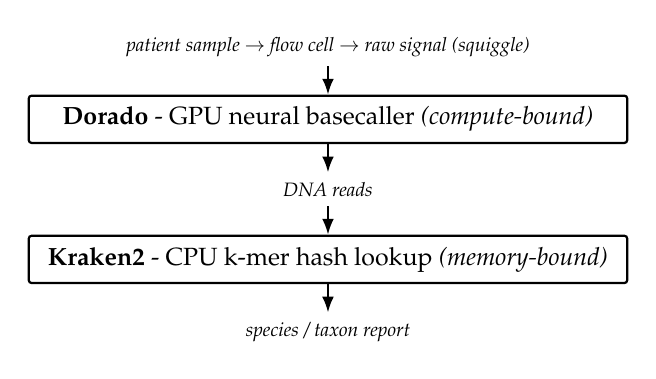
\begin{tikzpicture}[
  node distance=0.36cm and 0cm,
  box/.style={draw=inkblack, thick, rectangle, rounded corners=1pt, minimum width=7.6cm, minimum height=0.6cm, align=center, font=\small},
  lab/.style={font=\scriptsize\itshape, align=center},
  arr/.style={-{Latex[length=2mm]}, thick}
]
\node[lab] (n0) {patient sample $\rightarrow$ flow cell $\rightarrow$ raw signal (squiggle)};
\node[box, below=of n0] (n1) {\textbf{Dorado} - GPU neural basecaller \textit{(compute-bound)}};
\node[lab, below=of n1] (n2) {DNA reads};
\node[box, below=of n2] (n3) {\textbf{Kraken2} - CPU k-mer hash lookup \textit{(memory-bound)}};
\node[lab, below=of n3] (n4) {species / taxon report};
\draw[arr] (n0) -- (n1); \draw[arr] (n1) -- (n2); \draw[arr] (n2) -- (n3); \draw[arr] (n3) -- (n4);
\end{tikzpicture}
\end{center}

\subsection{Objective}
\begin{itemize}[nosep,leftmargin=1.4em]
  \item locate the true bottleneck of the pipeline through profiling, and show that Kraken2 classification is \textbf{memory-latency-bound}, not compute-bound.
  \item establish the database \textbf{memory footprint} - not thread count or arithmetic - as the primary optimisation lever, across server, edge, and desktop hardware.
  \item \textbf{halve} the footprint of a six-organism ESKAPE database by narrowing the CHT cell width, \textbf{without changing classification results}.
  \item \textbf{prove}, analytically and empirically, exactly which cell widths preserve accuracy (a lossless drop-in) and which require a confidence threshold.
\end{itemize}

% ================= SECTION 2 : ANALYSIS =================
\section{Analysis}

both pipeline stages were profiled on the ``Luna'' server, then characterised across three machines spanning a 35$\times$ range of last-level cache (Table~\ref{tab:testbed}). because reads and databases are identical across machines, classification percentages are hardware-independent; only speed and the scaling ceiling change.

\begin{table}[h!]
\centering\footnotesize
\caption{Test bed. Three machines spanning a 35$\times$ range of last-level cache (LLC).}
\label{tab:testbed}
\begin{adjustbox}{max width=\textwidth}
\begin{tabular}{@{}llll@{}}
\toprule
\textbf{Machine} & \textbf{Role} & \textbf{Key spec} & \textbf{Cache (LLC)} \\
\midrule
Luna & server & Xeon Platinum 8468, 96c/192t, 2$\times$ NVIDIA L40S & 210\,MB \\
Orion & edge device & Jetson AGX Orin, ARM Cortex-A78AE, 12c & 6\,MB \\
Desktop (OptiPlex 5090) & CPU workstation & Core i7-11700, 8c/16t & 16\,MB \\
\bottomrule
\end{tabular}
\end{adjustbox}
\end{table}

\subsection{The bottleneck: Dorado compute-bound, Kraken2 memory-bound}
several independent tools converge on one unambiguous split (Table~\ref{tab:evidence}). Dorado holds its GPU compute-saturated and its CPU idle, so no CPU tuning helps it. Kraken2 is the mirror image: a \code{cachegrind}~\cite{valgrind} attribution shows one function, \code{CompactHashTable::Get()}, runs only 0.65\% of instructions yet causes 96.24\% of all LLC read misses. each probe is a $\sim$100\,ns round trip to DRAM issued one at a time; the 8\,GB database is $\approx$38$\times$ Luna's 210\,MB LLC and $\approx$500$\times$ a 16\,MB desktop L3, so a miss is essentially guaranteed on every lookup. crucially the DRAM bus stays nearly idle ($\sim$10\,GB/s of 51): the CPU is not moving too much data, it is \textit{waiting too long} for each small request~\cite{roofline}. the correct lever is the database's \textbf{memory footprint}.

\begin{table}[h!]
\centering\footnotesize
\caption{Convergent evidence that Dorado is compute-bound and saturated while Kraken2 is memory-latency-bound.}
\label{tab:evidence}
\begin{adjustbox}{max width=\textwidth}
\begin{tabular}{@{}p{1.9cm}p{1.5cm}p{8.3cm}p{2.4cm}@{}}
\toprule
\textbf{Tool} & \textbf{Machine} & \textbf{Finding} & \textbf{Verdict} \\
\midrule
nsys & Luna & Dorado fast: GEMM 30.8\% $+$ LSTM 27.5\% $+$ beam 14.8\% of GPU time; hac: LSTM 68.0\% & compute-bound \\
nvidia-smi dmon & Luna & SM utilisation 97.6\% (fast) / 99.5\% (hac), no inter-batch sag & saturated, at capacity \\
CUDA API trace & Luna & 96--99\% of CUDA API time is \code{cudaStreamSynchronize} - CPU idle, waiting on GPU & GPU-paced, no CPU slack \\
cachegrind & Luna & \code{CompactHashTable::Get()} $=$ 0.65\% of instructions but 96.24\% of LLC read misses (7.6\,GB db) & memory-latency-bound \\
gprof & Luna / Desktop & \code{Get()} dominates CPU time (23--81\% by sample); minimizer scan takes the rest & memory-bound \\
perf (uncore) & Desktop & peak DRAM read traffic $\sim$10\,GB/s of a $\sim$51\,GB/s ceiling ($<$25\%), flat with db size & latency, not bandwidth \\
perf stat & Desktop & clean 8-thread build: IPC 1.40, 15.91\% cache-miss rate & confirmed at the optimum too \\
\bottomrule
\end{tabular}
\end{adjustbox}
\end{table}

\begin{honestbox}{A measurement-methodology correction}
\code{gprof} requires a \code{-pg} instrumented build, and running \code{perf} against that same \code{-pg} binary collapsed IPC to 0.154 and inflated backend-bound to 95.6\% - an artefact of the instrumentation, not the workload. removing \code{-pg} restored IPC to the 1.1-1.7 range, an 8-10$\times$ swing. all headline hardware-counter numbers below come from clean, bare-metal builds.
\end{honestbox}

\begin{figure}[h!]
\centering
\begin{adjustbox}{max width=\textwidth}
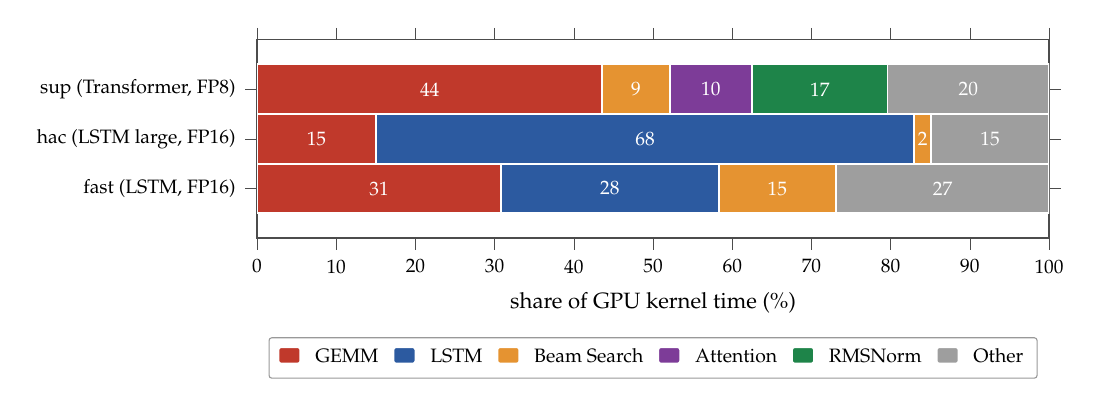
\begin{tikzpicture}
\definecolor{kGEMM}{HTML}{C0392B}\definecolor{kLSTM}{HTML}{2C5AA0}%
\definecolor{kBeam}{HTML}{E59331}\definecolor{kAttn}{HTML}{7D3C98}%
\definecolor{kRMS}{HTML}{1E8449}\definecolor{kOther}{HTML}{9E9E9E}%
\begin{axis}[grayaxis, width=0.96\linewidth, height=4.1cm,
  xbar stacked, xmin=0, xmax=100, bar width=18pt,
  xlabel={share of GPU kernel time (\%)},
  symbolic y coords={fast, hac, sup}, ytick=data,
  yticklabels={{fast (LSTM, FP16)},{hac (LSTM large, FP16)},{sup (Transformer, FP8)}},
  y tick label style={font=\scriptsize}, enlarge y limits=0.5,
  point meta=explicit symbolic,
  every node near coord/.append style={font=\scriptsize, text=white, inner sep=1pt},
  legend style={at={(0.5,-0.5)}, anchor=north, legend columns=6, column sep=3pt}, grid=none]
\addplot[fill=kGEMM,draw=white,line width=0.7pt,nodes near coords]
  coordinates {(30.8,fast)[31] (15.0,hac)[15] (43.6,sup)[44]};
\addplot[fill=kLSTM,draw=white,line width=0.7pt,nodes near coords]
  coordinates {(27.5,fast)[28] (68.0,hac)[68] (0,sup)[0]};
\addplot[fill=kBeam,draw=white,line width=0.7pt,nodes near coords]
  coordinates {(14.8,fast)[15] (2.1,hac)[2] (8.5,sup)[9]};
\addplot[fill=kAttn,draw=white,line width=0.7pt,nodes near coords]
  coordinates {(0,fast)[0] (0,hac)[0] (10.4,sup)[10]};
\addplot[fill=kRMS,draw=white,line width=0.7pt,nodes near coords]
  coordinates {(0,fast)[] (0,hac)[] (17.1,sup)[17]};
\addplot[fill=kOther,draw=white,line width=0.7pt,nodes near coords]
  coordinates {(26.9,fast)[27] (14.9,hac)[15] (20.4,sup)[20]};
\legend{GEMM, LSTM, Beam Search, Attention, RMSNorm, Other}
\end{axis}
\end{tikzpicture}
\end{adjustbox}
\caption{Dorado GPU kernel composition per model (Luna L40S, 104{,}918 reads). The dominant kernel shifts with architecture, yet all three keep the GPU compute-bound.}
\label{fig:kernels}
\end{figure}

\subsection{Thread scaling: the memory wall}
sweeping thread count on two machines gives the same shape - performance is capped by the memory system before cores run out (Table~\ref{tab:threads}). cache-miss \textit{count} on the desktop sweep is roughly constant ($\approx$375-400\,M) across thread counts; the miss \textit{rate} drifts only because the reference count grows, a ratio artefact. the ``8-thread sweet spot'' recurs on every CPU-only machine and, with Luna's 32-thread NUMA-pinned result, states the same conclusion at two scales.

\begin{table}[h!]
\centering\footnotesize
\caption{Thread-scaling findings. Parallelism is bounded by the memory hierarchy, not by free cores.}
\label{tab:threads}
\begin{adjustbox}{max width=\textwidth}
\begin{tabular}{@{}p{2.0cm}p{5.9cm}p{6.6cm}@{}}
\toprule
\textbf{Machine} & \textbf{Configuration} & \textbf{Effect} \\
\midrule
Luna\newline (96 cores) & sweep to 96 threads, NUMA-pinned to one local memory node & cache-resident panels scale near-linearly to a \textbf{32-thread sweet spot} ($\sim$21$\times$); multi-GB databases are DRAM-bound from 1T and plateau at 3--5$\times$ \\
Desktop\newline (8c/16t) & sweep 1--16 threads; retired instructions flat ($\pm$1.8\%) & stall cycles flat 1--8 threads, then \textbf{+13.9\% at 10}, \textbf{+24.5\% at 16}; the cliff appears in IPC, backend-bound and fetch-stalls at once \\
Desktop\newline (8c/16t) & optimal operating point & \textbf{8 threads}: 5.36$\times$ speedup, IPC 1.40, 74.6\% backend-bound; 16 threads adds only $\sim$23\% throughput while IPC drops $\sim$20\% \\
\bottomrule
\end{tabular}
\end{adjustbox}
\end{table}

\subsection{Database size, accuracy, and the cache cliff}
six databases were tested, from a 50\,MB custom ESKAPE panel to a 103\,GB gold-standard RefSeq database (Table~\ref{tab:detection}). detection and cache pressure rise together (Fig.~\ref{fig:dbsize}): adding organisms raises accuracy but also raises the LLC miss rate. there is a \emph{cache cliff} - Luna's 210\,MB LLC holds the 50\,MB panel whole (14.6\% miss, near-linear scaling), while every database above 142\,MB exceeds it and the miss rate climbs past 80\%; Orion's 6\,MB cache never reaches a pre-cliff point at all. the clinical stakes are concrete: the ESKAPE-only 142\,MB database assigns nearly all classified reads to \textit{P.\,aeruginosa} (0\% \textit{E.\,coli}/\textit{K.\,pneumoniae}) because it lacks those references, whereas the true sample is polymicrobial ($\sim$31--35\% \textit{P.\,aeruginosa}, $\sim$14--16\% \textit{E.\,coli}, $\sim$5\% \textit{K.\,pneumoniae}). yet a \textbf{focused panel} is not simply worse: the 51\,MB 6-genome database reaches 84.8\% (hac), within 11-12\,pp of the 7.6\,GB standard database at 1/150th the size, pinning calls cleanly at species level - the best detection-per-MB when the organisms are known. this is precisely why a smaller \emph{cell} (Section~3) matters most on commodity hardware.

\begin{table}[h!]
\centering\footnotesize
\caption{Detection (classified\%) by database and basecaller quality (hardware-independent).}
\label{tab:detection}
\begin{adjustbox}{max width=\textwidth}
\begin{tabular}{@{}lrrrr@{}}
\toprule
\textbf{Database} & \textbf{Size} & \textbf{fast} & \textbf{hac} & \textbf{sup} \\
\midrule
eskape\_51mb (custom, 6-genome) & 51\,MB & 80.94 & 84.80 & 85.40 \\
eskape\_650mb & 142\,MB & 61.77 & 65.28 & 65.87 \\
eskape\_human\_4gb & 3.8\,GB & 62.27 & 66.13 & 66.68 \\
standard\_8gb & 7.6\,GB & 82.66 & 95.77 & 97.09 \\
standard\_16gb & 15\,GB & 90.44 & 97.77 & 98.48 \\
pluspf\_103gb & 103.4\,GB & - & 98.86 & - \\
\bottomrule
\end{tabular}
\end{adjustbox}
\end{table}

\begin{figure}[h!]
\centering
\begin{adjustbox}{max width=\textwidth}
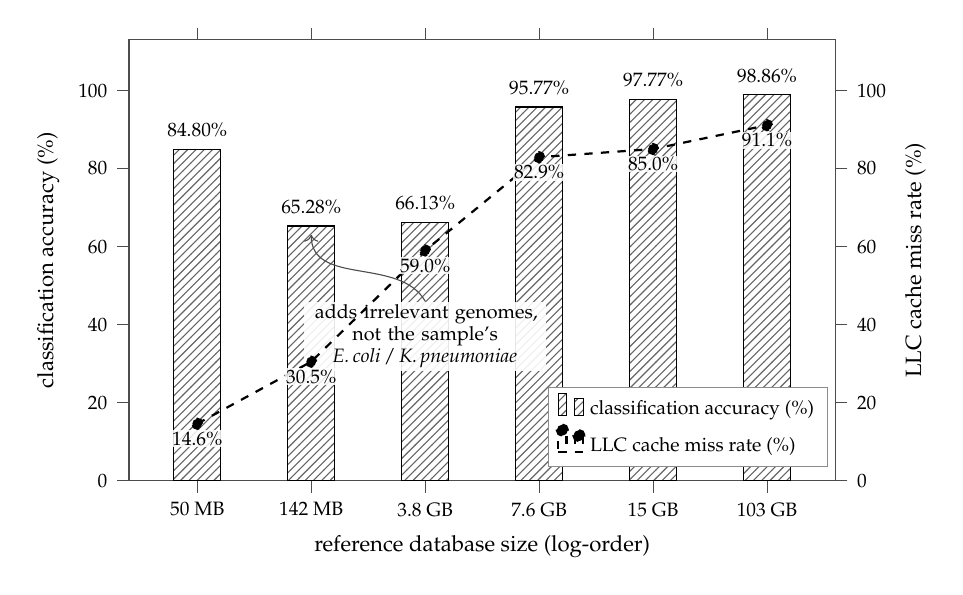
\begin{tikzpicture}
\begin{axis}[
  name=accax, width=0.74\linewidth, height=5.6cm, scale only axis,
  ybar, bar width=17pt, enlarge x limits=0.12,
  symbolic x coords={50 MB,142 MB,3.8 GB,7.6 GB,15 GB,103 GB}, xtick=data,
  xlabel={reference database size (log-order)}, ylabel={classification accuracy (\%)},
  ymin=0, ymax=113, ytick={0,20,40,60,80,100},
  tick align=outside, tick style={draw=black!70},
  axis line style={draw=black!70,line width=.5pt},
  label style={font=\footnotesize}, tick label style={font=\scriptsize},
  point meta=explicit symbolic, nodes near coords,
  every node near coord/.append style={font=\scriptsize, anchor=south, yshift=1pt},
  legend style={at={(0.99,0.03)}, anchor=south east, font=\scriptsize, legend cell align=left, draw=black!45},
  grid=none]
\addplot[pattern=north east lines, pattern color=black!60, draw=black]
  coordinates {(50 MB,84.80)[84.80\%] (142 MB,65.28)[65.28\%] (3.8 GB,66.13)[66.13\%]
               (7.6 GB,95.77)[95.77\%] (15 GB,97.77)[97.77\%] (103 GB,98.86)[98.86\%]};
\addlegendentry{classification accuracy (\%)}
\addlegendimage{black, dashed, thick, mark=*, mark options={fill=black}}
\addlegendentry{LLC cache miss rate (\%)}
\node[align=center, font=\scriptsize, text width=3.0cm, fill=white, fill opacity=0.9,
      text opacity=1, inner sep=1pt] (an) at (axis cs:3.8 GB,37)
  {adds irrelevant genomes, not the sample's \emph{E.\,coli}\,/\,\emph{K.\,pneumoniae}};
\draw[->, thin, black!70] (an.north) to[out=120,in=-90] (axis cs:142 MB,63);
\end{axis}
\begin{axis}[
  at=(accax.south west), anchor=south west,
  width=0.74\linewidth, height=5.6cm, scale only axis, enlarge x limits=0.12,
  symbolic x coords={50 MB,142 MB,3.8 GB,7.6 GB,15 GB,103 GB}, xtick=data, xticklabels={},
  axis x line=none, axis y line*=right,
  ymin=0, ymax=113, ytick={0,20,40,60,80,100},
  tick align=outside, tick style={draw=black!70},
  y axis line style={draw=black!70,line width=.5pt},
  ylabel={LLC cache miss rate (\%)},
  label style={font=\footnotesize}, tick label style={font=\scriptsize}]
\addplot[black, dashed, thick, mark=*, mark options={fill=black,scale=0.9},
  point meta=explicit symbolic, nodes near coords,
  every node near coord/.append style={font=\scriptsize, anchor=north, yshift=-2pt,
    fill=white, fill opacity=0.85, text opacity=1, inner sep=0.5pt}]
  coordinates {(50 MB,14.6)[14.6\%] (142 MB,30.5)[30.5\%] (3.8 GB,59.0)[59.0\%]
               (7.6 GB,82.9)[82.9\%] (15 GB,85.0)[85.0\%] (103 GB,91.1)[91.1\%]};
\end{axis}
\end{tikzpicture}
\end{adjustbox}
\caption{Database size vs.\ classification accuracy (hatched bars, left axis) and LLC cache-miss rate (dashed line, right axis), on a real 104{,}918-read sample (Luna, \code{reads\_hac}). Both climb with database size; the 142\,MB and 3.8\,GB databases add irrelevant genomes without the sample's missing species (\emph{E.\,coli}, \emph{K.\,pneumoniae}), dipping below the 50\,MB panel.}
\label{fig:dbsize}
\end{figure}

% ================= SECTION 3 : METHODOLOGY =================
\section{Methodology: Compact-Hash Cell-Width Reduction}

\subsection{Implementation}
a canonical ESKAPE panel spans only 35 taxonomy nodes, needing just \code{value\_bits}$=6$; the stock 32-bit cell spends the remaining 26 bits collision-checking a panel that does not need them. two narrower cells - \code{CompactHashCell16} (2\,B, 10/6) and \code{CompactHashCell24} (3\,B, 18/6) - were added to Kraken2's already-templated \code{CompactHashTable}, following its existing 40-bit cell. the width is chosen at build time (\code{-C \{16|24|32|40\}}), written self-describing into the header, and auto-detected on load; the hot path \code{Get()} is width-generic, so no classify-time flag is needed. the lookup and the implemented change are shown in Fig.~\ref{fig:flow}: a false positive can arise \emph{only} at the \code{key\_bits} comparison, so it is governed entirely by cell width.

\begin{figure}[h!]
\centering
\begin{adjustbox}{max width=\textwidth}
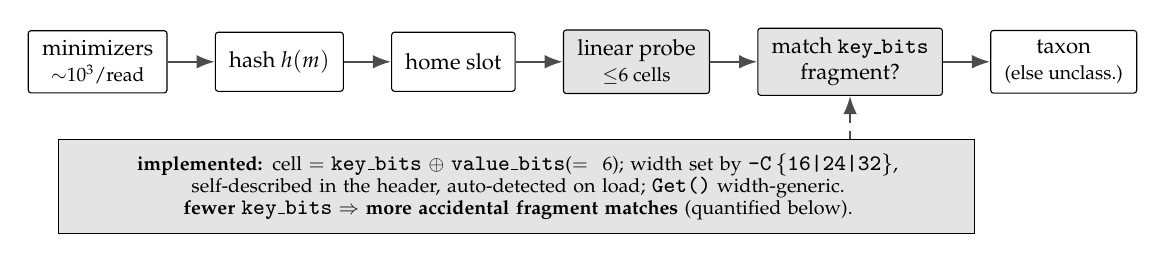
\begin{tikzpicture}[font=\footnotesize, >=Latex, every node/.style={align=center},
  proc/.style={draw=inkblack, rounded corners=1pt, minimum height=7.5mm, inner xsep=5pt, fill=white},
  key/.style={draw=inkblack, rounded corners=1pt, minimum height=7.5mm, inner xsep=5pt, fill=lightgray},
  ar/.style={->, thick, draw=black!70}]
\node[proc] (mini) {minimizers\\{\scriptsize$\sim$10$^3$/read}};
\node[proc, right=6mm of mini] (hash) {hash $h(m)$};
\node[proc, right=6mm of hash] (slot) {home slot};
\node[key,  right=6mm of slot] (probe) {linear probe\\{\scriptsize$\le$6 cells}};
\node[key,  right=6mm of probe] (cmp) {match \code{key\_bits}\\fragment?};
\node[proc, right=6mm of cmp] (out) {taxon\\{\scriptsize(else unclass.)}};
\draw[ar] (mini)--(hash); \draw[ar] (hash)--(slot); \draw[ar] (slot)--(probe);
\draw[ar] (probe)--(cmp); \draw[ar] (cmp)--(out);
\node[draw=inkblack, fill=lightgray, below=6mm of slot, xshift=8mm,
      text width=0.93\linewidth, inner sep=5pt, font=\scriptsize] (ann)
  {\textbf{implemented:} cell $=$ \code{key\_bits} $\oplus$ \code{value\_bits}($=6$); width set by \code{-C\,\{16|24|32\}},
   self-described in the header, auto-detected on load; \code{Get()} width-generic. \textbf{fewer \code{key\_bits} $\Rightarrow$ more accidental fragment matches} (quantified below).};
\draw[ar, dashed] (ann.north-|cmp) -- (cmp.south);
\end{tikzpicture}
\end{adjustbox}
\caption{Lookup mechanism and the implemented change. False positives arise only at the \code{key\_bits} comparison, so they are governed entirely by cell width.}
\label{fig:flow}
\end{figure}

\subsection{Proving the objective: an exponential false-positive law}
the objective is a footprint cut \emph{without changing answers}. Kraken2 stores only a \code{key\_bits}-wide hash \textit{fragment} ($b$), not the full minimizer, so two distinct minimizers can match by chance. with a linear-probing chain of expected length $p$ (Knuth~\cite{knuth}, at load factor $\alpha$), the per-minimizer false-positive rate and its amplification over the $N\!\approx\!10^3$ minimizers of a long read are
\begin{equation}
\mathrm{FP}_{\text{min}} \approx p\,2^{-b},\qquad
p \approx \tfrac12\!\left(1+\tfrac{1}{(1-\alpha)^2}\right)\Big|_{\alpha=0.70}\!\!\approx 6,\qquad
\mathrm{FP}_{\text{read}} \approx N\,p\,2^{-b}.
\label{eq:fp}
\end{equation}
each removed bit \emph{doubles} $\mathrm{FP}$ (Table~\ref{tab:fplaw}). a foreign read is mislabelled once $\mathrm{FP}_{\text{read}}\!\gtrsim\!1$; solving $N p\,2^{-b^\star}\!=\!1$ gives a sharp \textbf{cliff} at
\begin{equation}
b^\star = \log_2(Np) \approx \log_2(6000) \approx \mathbf{13}\ \text{check bits.}
\label{eq:cliff}
\end{equation}
this \emph{proves} the objective: 24-bit ($b{=}18$) and 32-bit ($b{=}26$) sit above the cliff and are indistinguishable, so \textbf{24-bit is a lossless, drop-in $-25\%$ footprint cut}; 16-bit ($b{=}10$) sits below it and must be rescued by a confidence threshold. narrowing the \emph{cell} leaves $\alpha$, $p$ and $b$-per-taxon untouched - only cutting \emph{capacity} would raise $\alpha$ and blow up both $p$ and $\mathrm{FP}$ (Table~\ref{tab:load}), so cell-narrowing is the correct lever.

\begin{table}[h!]
\centering\footnotesize
\begin{minipage}[t]{0.44\textwidth}\centering
\begin{tabular}{@{}rrl@{}}
\toprule
\textbf{fill $\alpha$} & \textbf{$p$} & \textbf{note} \\
\midrule
50\% & 2.5 & cheap \\
\textbf{70\%} & \textbf{6.1} & \textbf{our DB} \\
80\% & 13 & rising \\
90\% & 50 & slow \\
95\% & 200 & very slow \\
\bottomrule
\end{tabular}
\captionof{table}{Probe length vs load~\cite{knuth}.}
\label{tab:load}
\end{minipage}\hfill
\begin{minipage}[t]{0.52\textwidth}\centering
\begin{tabular}{@{}lrrl@{}}
\toprule
\textbf{cell} & \textbf{$b$} & \textbf{FP / minimizer} & \textbf{FP / read} \\
\midrule
32-bit & 26 & 1 in 11\,M & $\sim$10$^{-4}$ \\
24-bit & 18 & 1 in 44\,k & $\sim$0.02 \\
16-bit & 10 & 1 in 170  & $\sim$6 \\
\bottomrule
\end{tabular}
\captionof{table}{Eq.~\eqref{eq:fp}: below $b^\star\!\approx\!13$, FP/read $>1$.}
\label{tab:fplaw}
\end{minipage}
\end{table}

% ================= SECTION 4 : RESULTS =================
\section{Results}

applying the method to the ESKAPE panel confirms Eq.~\eqref{eq:cliff} exactly. \emph{24-bit reproduces 32-bit bit-for-bit} at every threshold, giving a free 25\% footprint cut; \emph{16-bit halves the database} but over-classifies via collisions until a small threshold is applied. the footprint scales exactly with cell width (Table~\ref{tab:cellwidth}, byte-verified): 48.80\,MB $\to$ 36.60\,MB ($-25\%$) $\to$ 24.40\,MB ($-50\%$), all holding the same 8.53\,M minimizers at $\sim$70\% load.

\begin{table}[h!]
\centering\footnotesize
\caption{Cell-width trade-off, byte-verified (32\,B header $+$ capacity $\times$ cell-bytes).}
\label{tab:cellwidth}
\begin{adjustbox}{max width=\textwidth}
\begin{tabular}{@{}lrrl@{}}
\toprule
\textbf{Cell width} & \textbf{Size} & \textbf{Deviation from 32-bit ($T{=}0$)} & \textbf{Runtime requirement} \\
\midrule
32-bit (stock) & 48.80\,MB & baseline & - \\
24-bit & 36.60\,MB ($-$25\%) & $+$0.3--0.45\% & none (drop-in) \\
16-bit & 24.40\,MB ($-$50\%) & $+$16--21\% & $-$T $\geq$ 0.05 mandatory \\
\bottomrule
\end{tabular}
\end{adjustbox}
\end{table}

correctness is bit-identical for legitimate hits (self-classifying the six genomes calls each organism's own species identically; \code{dump\_table} round-trips the same 35 taxa for all three widths). the 16-bit deviation is provably a collision artefact, not signal: it produces cross-phylum hits impossible under exact k-mer matching (Fig.~\ref{fig:inflation}), inflating Gram-positive \textit{S.\,aureus} $\times$48 and \textit{E.\,faecium} $\times$1476 with reads sharing no real 31-mers, and at a common capacity the 16-bit table holds 9{,}626 fewer occupied cells than 32-bit - distinct minimizers merging under the narrower key. a threshold of \code{-T 0.05} collapses the 16-bit deviation to $<$0.6\%; 24-bit needs none.

\begin{figure}[h!]
\centering
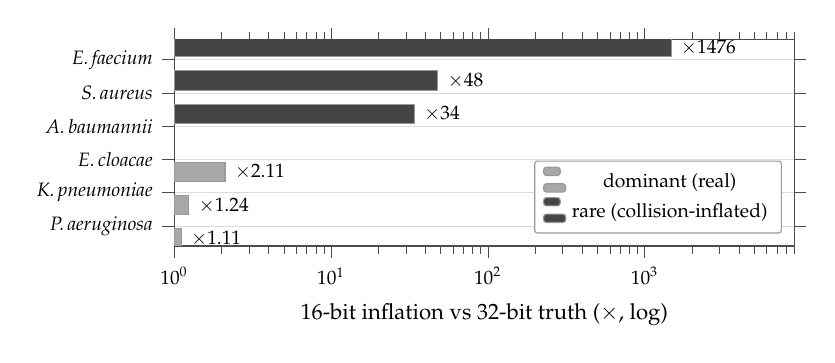
\begin{tikzpicture}
\begin{axis}[grayaxis, width=0.78\linewidth, height=4.2cm,
  xmode=log, xmin=1, xmax=9000,
  xlabel={16-bit inflation vs 32-bit truth ($\times$, log)},
  ytick={1,2,3,4,5,6},
  yticklabels={{\itshape P.\,aeruginosa},{\itshape K.\,pneumoniae},{\itshape E.\,cloacae},%
               {\itshape A.\,baumannii},{\itshape S.\,aureus},{\itshape E.\,faecium}},
  y tick label style={font=\scriptsize}, ymin=0.4, ymax=6.6,
  xbar, bar width=7pt, xmajorgrids=false,
  legend style={at={(0.98,0.06)}, anchor=south east, font=\scriptsize}]
\addplot[fill=g2,draw=black!40, nodes near coords, point meta=explicit symbolic,
  every node near coord/.append style={font=\scriptsize, anchor=west}]
  coordinates {(1.11,1)[$\times$1.11] (1.24,2)[$\times$1.24] (2.11,3)[$\times$2.11]};
\addplot[fill=g5,draw=black!40, nodes near coords, point meta=explicit symbolic,
  every node near coord/.append style={font=\scriptsize, anchor=west}]
  coordinates {(34,4)[$\times$34] (48,5)[$\times$48] (1476,6)[$\times$1476]};
\legend{dominant (real), rare (collision-inflated)}
\end{axis}
\end{tikzpicture}
\caption{16-bit read-count inflation per species at $-T\,0$ (105\,k \code{reads\_fast}). Abundant species barely move; rare Gram-positive species explode - a pure hash-collision signature (a larger 1.87\,M-read run showed the same, \textit{E.\,faecium} $\times$7{,}118).}
\label{fig:inflation}
\end{figure}

\subsection{Cross-hardware validation}
a 1{,}728-run desktop sweep (4 cell widths $\times$ 16 pod5 files $\times$ 9 thread counts $\times$ 3 runs) reproduces the $b^\star\!\approx\!13$ cliff on data it was never fit to (Fig.~\ref{fig:cliff}, Table~\ref{tab:sweep}): 24-bit ($b{=}18$) matches 32-bit, 20-bit ($b{=}14$, just above) inflates only $+0.75$\,pp, and 16-bit ($b{=}10$, below) jumps $+7.2$\,pp. the sweep also confirms the latency picture: peak DRAM traffic is $\sim$10\,GB/s of a $\sim$51\,GB/s ceiling and \emph{falls} 8T$\to$16T while throughput rises; smaller cells lower the miss rate and raise IPC, so the accurate 24-bit build is strictly cheaper as well as smaller. \textbf{recommendation: 24-bit as the no-conditions default; 16-bit with \code{-T 0.05} where footprint is the binding constraint.}

\begin{figure}[h!]
\centering
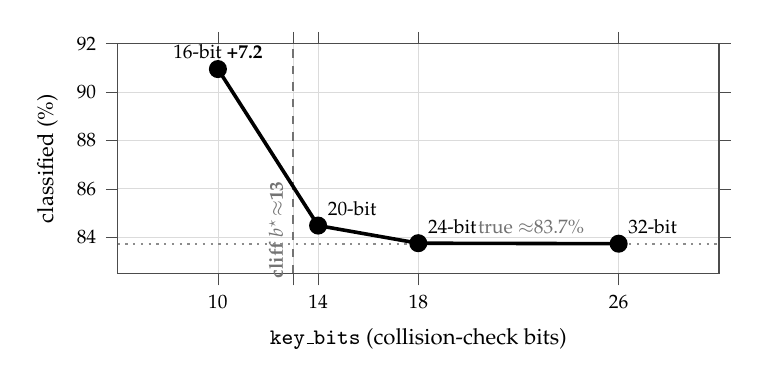
\begin{tikzpicture}
\begin{axis}[grayaxis, width=0.76\linewidth, height=4.5cm,
  xlabel={\code{key\_bits} (collision-check bits)}, ylabel={classified (\%)},
  xmin=6, xmax=30, ymin=82.5, ymax=92, xtick={10,13,14,18,26}, xticklabels={10,,14,18,26}, clip=false]
\addplot[dashed, black!55, line width=1pt, forget plot] coordinates {(13,82.5)(13,92)};
\node[black!55, font=\scriptsize\bfseries, anchor=south, rotate=90] at (axis cs:13,84.3) {cliff $b^\star\!\approx$13};
\addplot[dotted, black!45, line width=0.8pt, forget plot] coordinates {(6,83.73)(30,83.73)};
\node[black!55, font=\scriptsize, anchor=south west] at (axis cs:20,83.73) {true $\approx$83.7\%};
\addplot[black, mark=*, line width=1.3pt, mark size=2.6pt] coordinates {(10,90.95)(14,84.48)(18,83.75)(26,83.73)};
\node[font=\scriptsize, anchor=south] at (axis cs:10,90.95) {16-bit \textbf{+7.2}};
\node[font=\scriptsize, anchor=south west] at (axis cs:14,84.48) {20-bit};
\node[font=\scriptsize, anchor=south west] at (axis cs:18,83.75) {24-bit};
\node[font=\scriptsize, anchor=south west] at (axis cs:26,83.73) {32-bit};
\end{axis}
\end{tikzpicture}
\caption{The collision cliff, measured. Desktop classification vs check-bit count (1{,}728-run sweep): widths above $b^\star\!\approx\!13$ sit on the true rate; 16-bit falls off it - confirming Eq.~\eqref{eq:cliff}.}
\label{fig:cliff}
\end{figure}

\begin{table}[h!]
\centering\footnotesize
\caption{Per-cell means at 16 threads, 1{,}728-run desktop sweep.}
\label{tab:sweep}
\begin{adjustbox}{max width=\textwidth}
\begin{tabular}{@{}lrrrrrr@{}}
\toprule
\textbf{Cell} & \textbf{$b$} & \textbf{Classified\%} & \textbf{Cache-miss\%} & \textbf{LLC-miss\%} & \textbf{IPC} & \textbf{Speedup (16T)} \\
\midrule
32-bit & 26 & 83.73 & 60.99 & 58.58 & 1.12 & 8.1$\times$ \\
24-bit & 18 & 83.75 & 57.73 & 55.78 & 1.17 & 7.9$\times$ \\
20-bit & 14 & 84.48 & 57.68 & 55.28 & 1.17 & 8.0$\times$ \\
16-bit & 10 & 90.95 & 50.77 & 48.20 & 1.23 & 7.4$\times$ \\
\bottomrule
\end{tabular}
\end{adjustbox}
\end{table}

% ================= SECTION 5 : FUTURE WORK =================
\section{Future Work}

\begin{itemize}[nosep,leftmargin=1.4em]
  \item \textbf{Latency-hiding lookup cache (designed, not yet run).} both tracks independently designed the same next step: a small per-thread lookup cache that catches repeated k-mers before they reach the slow hash table (the summer track's \textit{thread-local cache}, designed with Prof.\ Kolin Paul; the \textit{kraken2opti} track's \textit{4-way set-associative LRU cache} wrapping \code{Get()}, projected at 9--12\% cache-miss rate and IPC 1.8--2.3). the summer track measured that \textbf{90.7\% of lookups within a run repeat a k-mer already seen} (32.8\,M unique of 351.8\,M total), far above the 20\% originally assumed, since clinical samples have a dominant species. combined with three smaller patches (AVX-512 vector flags, huge-page hints, and a one-line \code{\_\_builtin\_prefetch}), the summer track's baseline of 4.405\,s (32 threads, pinned) projects to roughly \textbf{3.0\,s (32\% cut)}, and with further micro-patches to \textbf{2.6\,s (41\% cut)}. \textbf{neither projection has been executed.} \code{run\_kraken2\_opt\_v1.sh} has never run against a patched binary; the \textit{kraken2opti} LRU cache is source-verified but unbuilt. this is the single highest-priority open item across both tracks, and the two designs should very likely be merged into one implementation rather than built twice.
  \item \textbf{Change the probing scheme to shrink $p$.} Eq.~\eqref{eq:fp} makes both false-positive rate and lookup cost proportional to the average probe length $p$. replacing linear probing with \textbf{double hashing} (or Robin-Hood / cuckoo hashing) cuts $p$ from $\approx$6 to $\approx$2.5 at the same 70\% load, which shifts the cliff $b^\star=\log_2(Np)$ down by $\approx1.3$ bits - making 16-bit safe without a threshold and opening a possible sub-16-bit cell. this needs only a change to \code{second\_hash()}, and its effect is directly predicted by the model above.
  \item \textbf{Bitmask cell.} a 6-bit-per-organism value so one \code{Get()} answers all panel members at once.
  \item \textbf{Coverage and upstreaming.} extend the panel to the missing ESKAPE member (\textit{A.\,baumannii}); upstream the 16/24-bit cells to mainline Kraken2 (five additive files plus one over-capacity guard); and re-run the sweeps on a $\geq$200\,MB-L3 server to test whether a large LLC lifts panel databases off the DRAM latency wall entirely.
\end{itemize}

{\footnotesize\textit{Reproducibility.} raw \code{perf}/\code{gprof}/\code{nsys}/\code{cachegrind} outputs, phase reports, and cell-size build artefacts are archived under \code{kraken2opti/} (\code{reports/}, \code{results/}); the 1{,}728-run sweep under \code{results/perf\_threadsweep/} and the cell-width sweeps under \code{results/eskape\_16bit/}.}

% ================= REFERENCES =================
\begin{thebibliography}{9}
\footnotesize
\bibitem{kraken2} D.\,E.\ Wood, J.\ Lu, and B.\ Langmead, ``Improved metagenomic analysis with Kraken 2,'' \textit{Genome Biology}, vol.\ 20, no.\ 1, p.\ 257, 2019.
\bibitem{kraken1} D.\,E.\ Wood and S.\,L.\ Salzberg, ``Kraken: ultrafast metagenomic sequence classification using exact alignments,'' \textit{Genome Biology}, vol.\ 15, no.\ 3, R46, 2014.
\bibitem{minimizers} M.\ Roberts, W.\ Hayes, B.\,R.\ Hunt, S.\,M.\ Mount, and J.\,A.\ Yorke, ``Reducing storage requirements for biological sequence comparison,'' \textit{Bioinformatics}, vol.\ 20, no.\ 18, pp.\ 3363--3369, 2004.
\bibitem{knuth} D.\,E.\ Knuth, \textit{The Art of Computer Programming, Vol.\ 3: Sorting and Searching}, 2nd ed. Reading, MA, USA: Addison-Wesley, 1998.
\bibitem{valgrind} N.\ Nethercote and J.\ Seward, ``Valgrind: a framework for heavyweight dynamic binary instrumentation,'' in \textit{Proc.\ ACM SIGPLAN PLDI}, 2007, pp.\ 89--100.
\bibitem{roofline} S.\ Williams, A.\ Waterman, and D.\ Patterson, ``Roofline: an insightful visual performance model for multicore architectures,'' \textit{Commun.\ ACM}, vol.\ 52, no.\ 4, pp.\ 65--76, 2009.
\bibitem{eskape} L.\,B.\ Rice, ``Federal funding for the study of antimicrobial resistance in nosocomial pathogens: no ESKAPE,'' \textit{J.\ Infect.\ Dis.}, vol.\ 197, no.\ 8, pp.\ 1079--1081, 2008.
\bibitem{dorado} Oxford Nanopore Technologies, ``Dorado: a basecaller for Oxford Nanopore reads,'' 2024. [Online]. Available: https://github.com/nanoporetech/dorado
\end{thebibliography}

\end{document}
